\documentclass{article}

\usepackage{graphicx}
\usepackage{multicol}
\usepackage{fullpage}
\usepackage{floatflt}
\usepackage{xspace}

\def\degC{$^{\circ}$C }
\def\degf{$^{\circ}$F }
\def\vol #1 {{\bf #1}, $\;\;$}
\def\refer{\par\noindent\hangindent\parindent\hangafter1}


\title{Herzmann Family Christmas Letter 2016}
\author{Daryl Herzmann${}^1$, Elizabeth Herzmann${}^1$, Margaret 
Herzmann${}^2$,\\
Robert Herzmann${}^3$, AND Charlotte Herzmann${}^4$ \\
\it{${}^1$ Caretakers},
\it{${}^2$ Senior Child},
\it{${}^3$ Middle Child},
\it{${}^4$ Soon to be Born Child}}
\date{17 December 2016}

\makeatletter
\newenvironment{tablehere}
  {\def\@captype{table}}
  {}

\newenvironment{figurehere}
  {\def\@captype{figure}}
  {}
\makeatother

\newcommand{\Line}[0]{%
  \rule{0cm}{0cm}\\\hrule\rule{0cm}{0cm}%
}

\addtolength{\textheight}{1.5in}

\begin{document}
\maketitle

\begin{abstract}
Last year's Christmas Letter correction of the 2014 Christmas Letter
(Herzmann et al., 2014) was well received, but disliked by the publisher
(Staples) due to light pen markings and razor tight page margins. After intense negotiation with the publisher, it was
decided to \textbf{not correct} the correction this year. So we hope this new
edition of the yearly Christmas Letter finds you sitting down and ready to
decipher.
\end{abstract}

\Line

\begin{multicols}{2}

\section{Introduction} 

The fact-checking reader will notice an additional co-author of this dossier
named Charlotte. She is not scheduled for departure from Mommy until 0245 AM CST 17
January 2017, but there is always hope that she comes early.  So for now, our
family constitutes four autonomous humans (Daryl "Daryl" (38), Elizabeth
"Liz"[also great with child] (32), Margaret "Miss Maggie" (3), and Robert
"Ro-Ro" (2)) and one cat (Snoopy (8)).

\subsection{Housing}

Our family continues to make our residence in upscale and increasingly
expensive Ankeny, Iowa.  This will be our final and only home so to spite our
real estate agent who predicted that we could move houses after seven years, due
to the \textit{seven year itch}.  We are about to replace two rottening upstairs
windows as a sign of our commitement to stay.  So continue to denote our address
in your address books with permanent marker.  Liz's, now both retired, parents
continue to live down the block from us, which is magical.

\subsection{Conveyances}

After numerous attempts of gerrymandering three car seats into the back row of
daryl's car, it was declared a failure by Miss Maggie.  So the three child
encumbrance requirement vacates it as a viable option going forward.  The
prospect of a two minvan household is terrifying, so other options will be
sought.  Next year's letter will provide the anxious reader with the result.

\begin{figurehere}
 \centering   
 \resizebox{.95\columnwidth}{!}{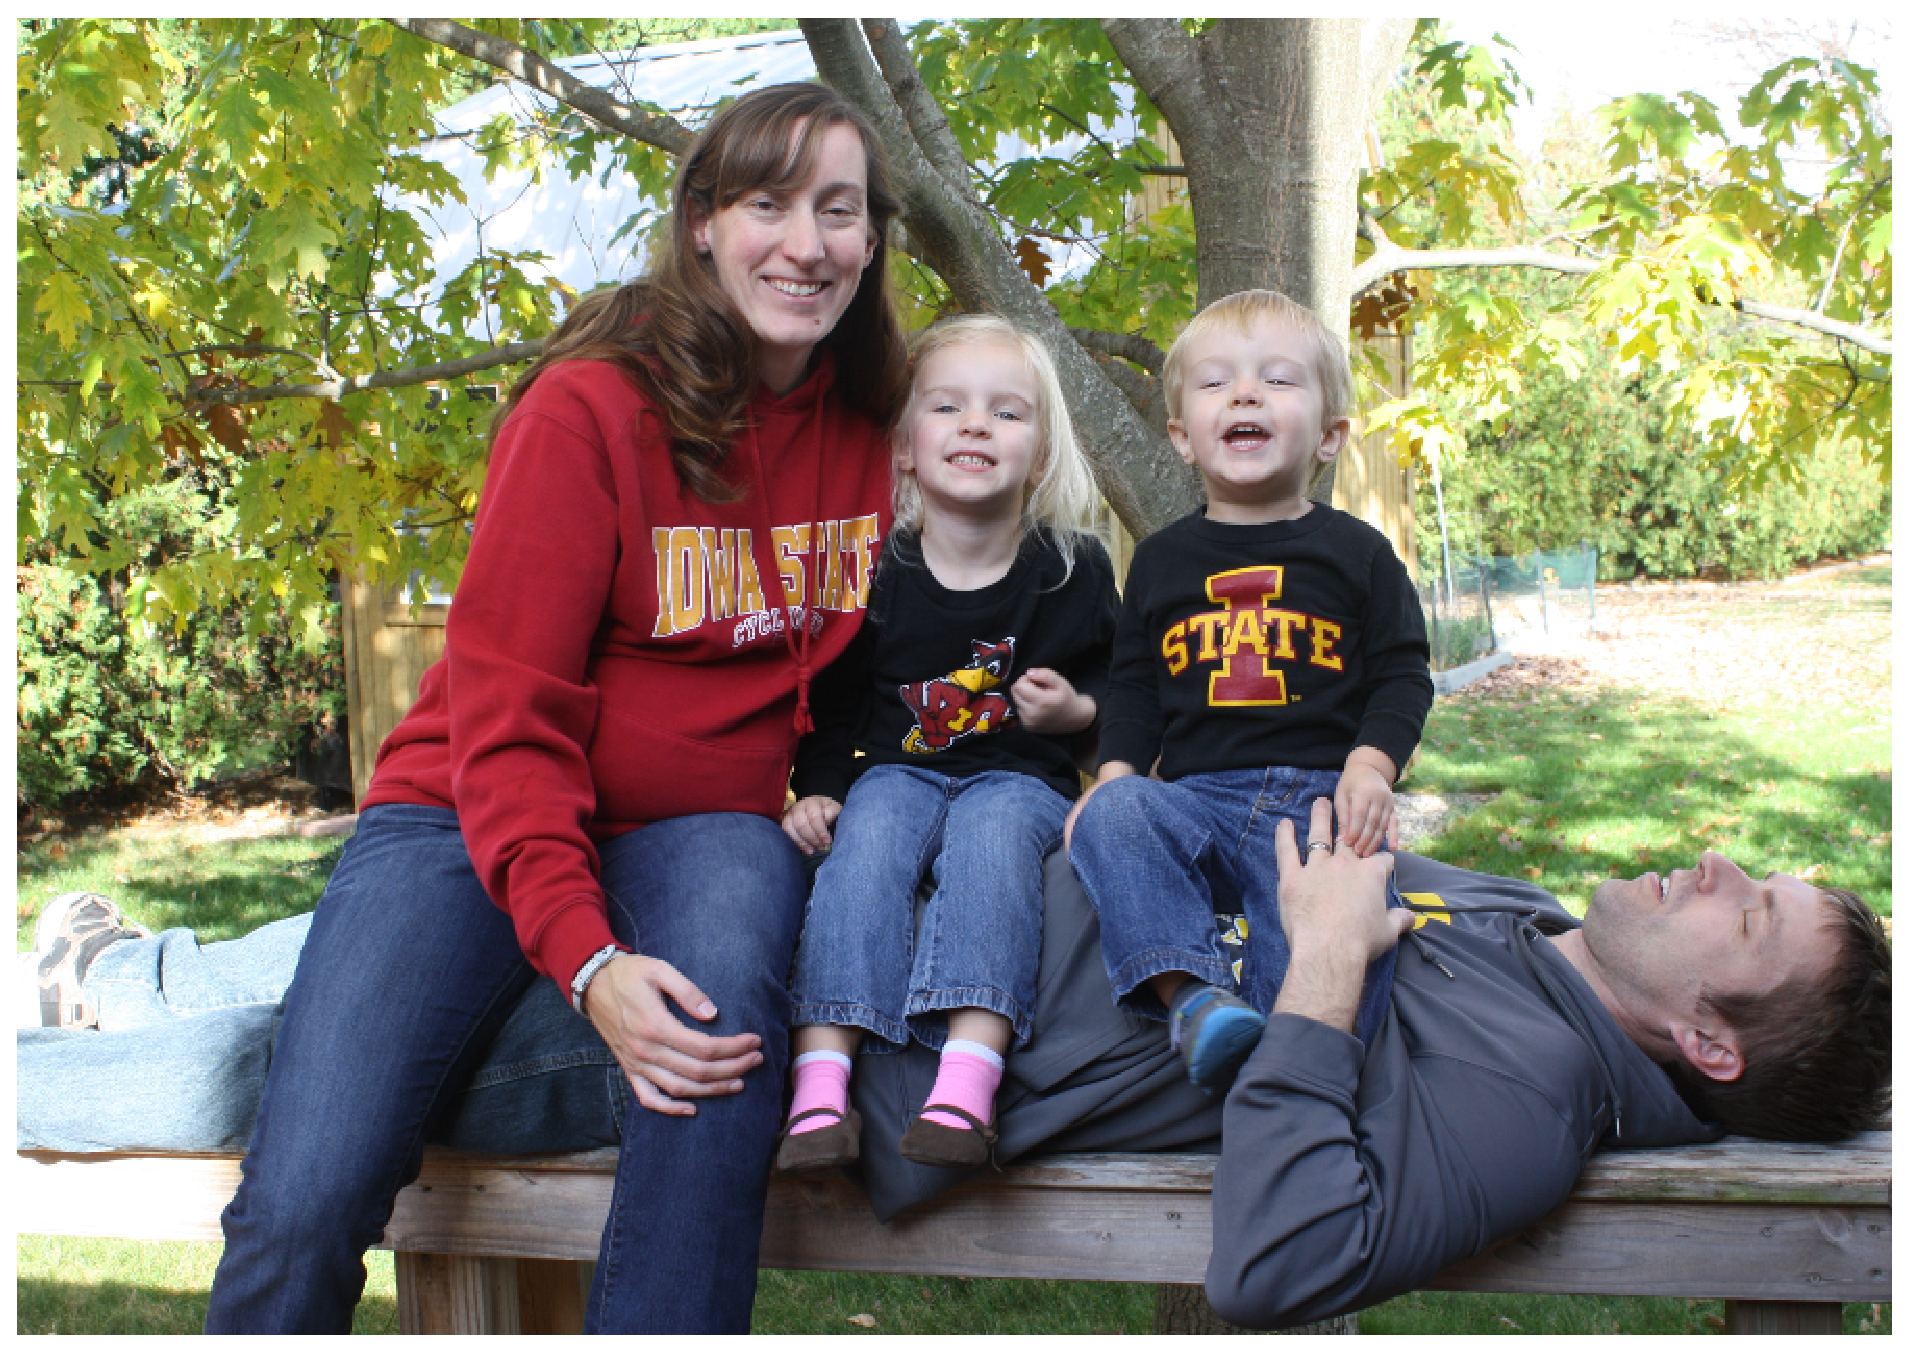
\includegraphics[angle=0]{plots/f1_2016.eps}}
 \caption{Representative depiction of daryl's support of the growing family.}
\end{figurehere}

\subsection{Employment}
Daryl remains employed with Iowa State University and continues to work on 
his weather data collection stuff.  Working at the University continues to be
great fun and his favorite activity is extorting grad students out of candy. He
joined an academic committee for a three year term that brings him to Boulder, 
Colorado twice per year for meetings.

Liz continues her work at Johnston Middle School with 8th and 9th graders. 
The Science Olympiad program, which Liz coaches, continues to flourish. 
Liz and her co-coach have expanded the program to the High school, which 
now supports about 45 additional students.  They prepare after school 
daily for the State competition in April.  Liz will again mentor a student 
teacher in the Spring.  Liz enjoys mommy - Maggie time on Saturday 
mornings with story time at the local library and summer swim lessons.

Miss Maggie's work detail involves feeding the cat daily.  Mr Robert is
unemployed.

\section{Miss Maggie}

When not being fussy, Miss Maggie is mostly pleasant to deal with.  She is very
much excited about the arrival of Charlotte and wants to do most of the child
rearing herself. We just hope that Charlotte is not born on Miss Maggie's
birthday (13 January) as that may cause a change in her disposition.  Miss
Maggie loves to do art and mostly able to inscribe her name on paper and/or walls.

This fall, Miss Maggie went with her daddy to Grandma Barb's farm to help the
neighbors with the corn harvest.  She thought riding in the big green John Deere
tractor with a cab was the greatest thing ever (Figure 2).  Grandma Barb's
tractor (cabless) '\textit{does not have a door}', so Miss Maggie instructed her
to purchase a new tractor with a door.  She was a good helper for the brief
while at home and did not want to get out of the tractor. She threw a large fit
when asked to ride in a red colored tractor.

\bigskip

\begin{figurehere}
 \centering   
 \resizebox{.95\columnwidth}{!}{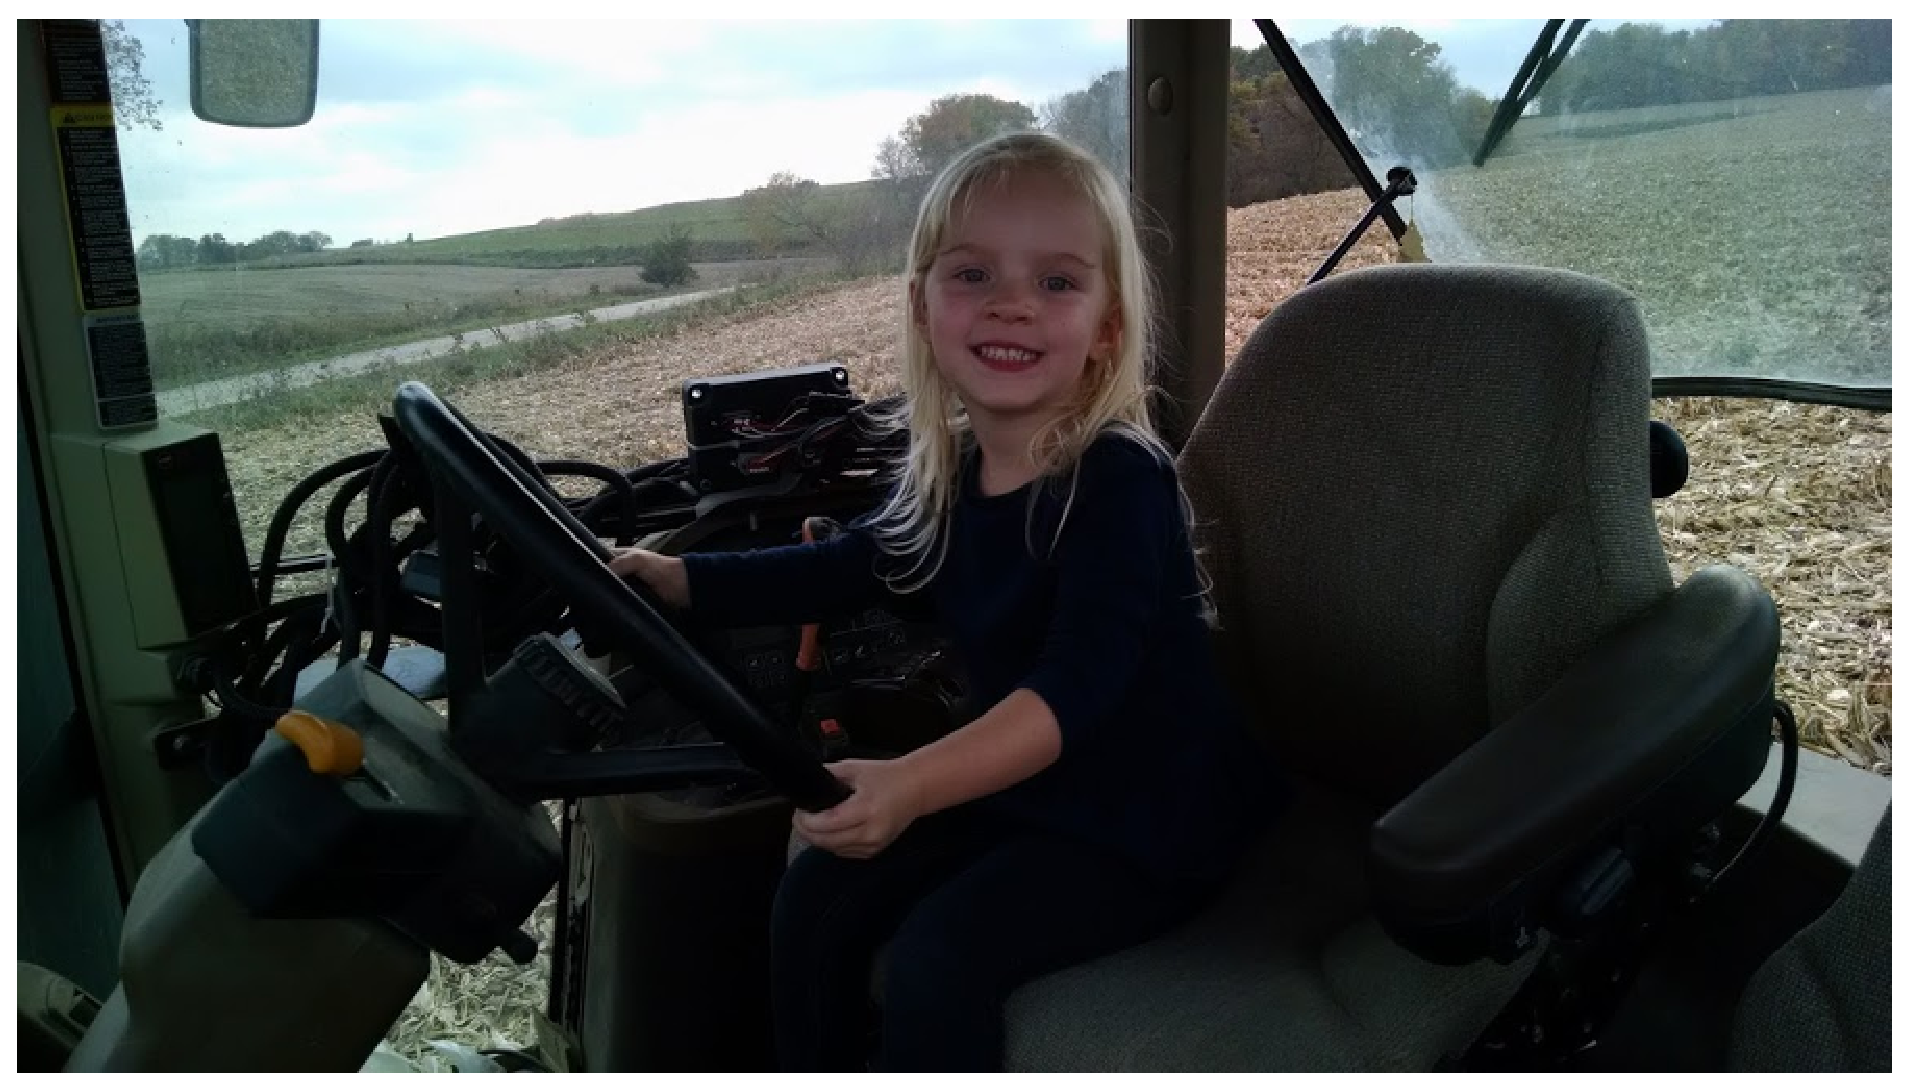
\includegraphics[angle=0]{plots/f3_2016.eps}}
 \caption{Miss Maggie safely driving her favorite tractor.}
\end{figurehere}

\section{Mr Robert}

Mr Robert is many handfuls of joy.  After the relative ease of raising Miss
Maggie, he has proven to be two orders of magnitude more challenging.  He now
shares a room with Miss Maggie and only recently has decided to sleep in his own
bed for the duration of the night. He seems to be an intelligent child, but has
a propensity of rearing back and raming his head into his unsuspecting parents. 

Mr Robert enjoys doing puzzles, eating pancakes or pizza, and wrestling with his
daddy after being told not to wrestle with pregnant mommy.  He is showing some
interest in potty training, but not ready to commit yet.

He is unsure about the arrival of Charlotte and after denoting the presence of a
baby in mommy's belly, he will left up his shirt to declare a baby in his belly
as well.  Once Charlotte gets bigger, he will move out of Maggie's room and back
into the nursery room with Charlotte joining Maggie.  Or maybe all three
children will be assigned to the same room to see what happens!

\begin{figurehere}
 \centering   
 \resizebox{.95\columnwidth}{!}{\includegraphics[angle=0]{plots/size.ps}}
 \caption{Actual and modeled family size.}
\end{figurehere}

\section{Summary}

Our family continues to grow in size (Figure 3) and love (Figure 4). Thankfully
the increases in love are non-linear as each child has brought our family
infinite joy.  As long as there is two of everything in the house, the children
need not fight.  We hope Charlotte does not require purchasing three of
everything to keep the peace!

\bigskip

\begin{figurehere}
 \centering   
 \resizebox{.95\columnwidth}{!}{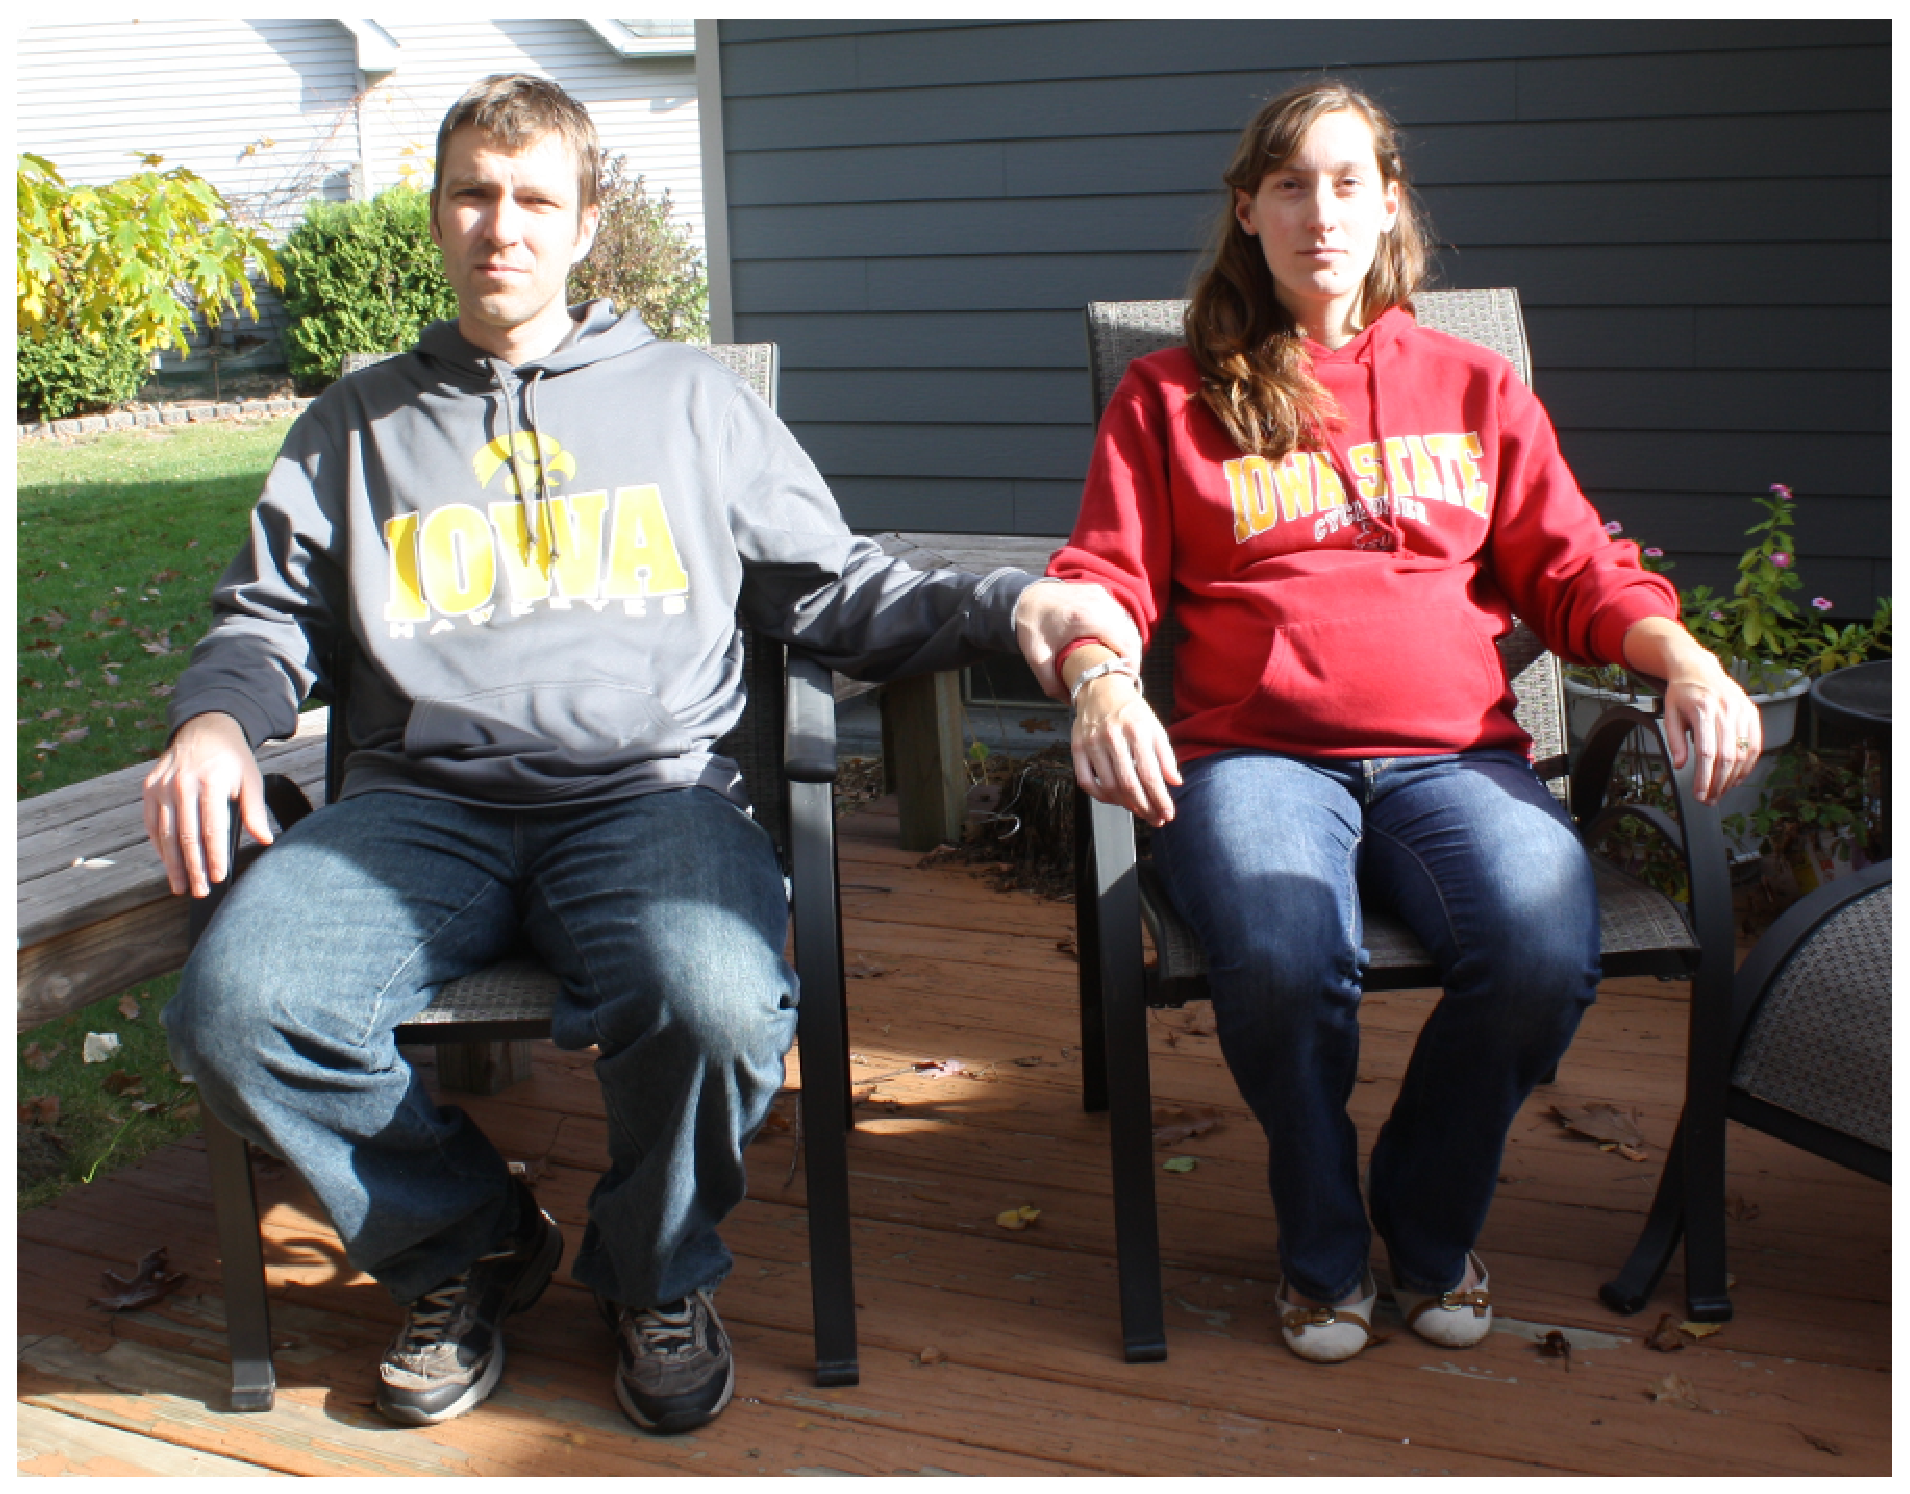
\includegraphics[angle=0]{plots/f2_2016.eps}}
 \caption{A candid and affectionate moment for a couple still very much in
 love.}
\end{figurehere}

\bigskip
  \emph{Acknowledgments} Our family wishes to thank you for the generous 
support, prayers, cards, gifts, and visits you have provided us in the past
year. With your continued support, this letter will be produced again
next year. Please note that the format chosen for this correspondence was
completely Daryl's idea and execution. Full \LaTeX\xspace source can be found on 
Daryl's github page.

\section{References}

\refer Github, 2016: https://github.com/akrherz/me , visited 17 Dec 2016.
\refer Herzmann, Daryl E., et al. Herzmann Family Christmas Letter 2014. 

\end{multicols}

\end{document}

